%!TEX program = xelatex 
\documentclass[11pt, a4paper]{scrartcl}
\usepackage[utf8]{inputenc}
%\usepackage[a4paper,lmargin={3.5cm},rmargin={3.5cm}, tmargin={2.5cm},bmargin = {2.5cm}]{geometry}
\usepackage{setspace}
\usepackage{indentfirst}
\usepackage{mathtools}
\usepackage{enumitem}
\usepackage{graphicx}
\usepackage{yfonts, amsmath, amssymb}
\usepackage[backend=biber, authordate, ibidtracker=context, natbib]{biblatex-chicago}
\usepackage{titlesec}
\usepackage{color}
\usepackage{tikz}
\usetikzlibrary{fit,positioning}
\usetikzlibrary{arrows}

\onehalfspacing{}

\addbibresource{bib.bib}

\usepackage{fontspec}
\newfontfamily\osfamily{Latin Modern Roman Demi}

\setkomafont{disposition}{\osfamily}

\renewcommand{\i}[1]{\emph{#1}}
\renewcommand{\L}{\mathcal{L}}
\renewcommand{\v}[1]{\vec{\mathrm{#1}}}

\newcommand{\m}[1]{\textswab{#1}}
\newcommand{\given}[1][]{\:#1\vert\:}


\titleformat{\section}[block]{\Large\bfseries\osfamily\filcenter}{}{1em}{}
%\titleformat{\section}{\Large\bfseries\osfamily}{\thesection}{1em}{}
\titleformat{\subsection}[block]{\large\filcenter}{}{1em}{}
%\titleformat{\subsection}{\large\bfseries\osfamily}{\thesubsection}{1em}{}
%\renewcommand{\thesection}{\Roman{section}} 

\title{\osfamily{}Learning Imprecise Information}
\author{Class Paper for Central Topics in Philosophy of Science \\ Prof.\ Dr.\ Stephan Hartmann \\ WS 2017/2018, LMU Munich \\ Conrad Friedrich \\ \texttt{conradfriedrich@posteo.net} \\ Word count: 3001}

\begin{document}

\maketitle
\thispagestyle{empty}
%\tableofcontents
\newpage
\section{I}
Modeling the cognitive state and dynamics of epistemic agents to research predominantly normative issues is a central aspect in the philosophy of science and formal epistemology. In particular, it is crucial to tell a coherent and convincing story about reasoning with uncertain and incomplete information. The all-too-pervasive problem of induction reappears here, too. A crowd favorite in much of these fields is the use of a Bayesian framework, which has proven meaningfully relevant, versatile, and successful (e.g. \citet{Bovens2003-HARBE}, \citet{Hartmann2017}). So much so that it is not improper to speak of something like a Bayesian orthodoxy in the philosophy of science. It is very common to assess questions about evidence and uncertain reasoning within the Bayesian framework, implying the use of the mathematical theory of probabilities to capture doxastic states and reasoning processes of epistemic agents.

The Bayesian framework is an important element in the philosopher's toolbox. The framework forces her to very precisely state her problem in a quantifiable manner, and repays this effort with the deductive capabilities of probability theory. When such a powerful tool becomes orthodoxy, it might be tempting to disregard the substantial assumptions made just to be able to apply the tool. When you've got a hammer, everything looks like a nail. The method should not be implemented for its own sake, of course, and instead be regulated by some sensible desiderata for successful use. This has been much-discussed, but two particularly relevant desiderata are somewhat self-evident: (i) The lack of complexity of the framework. Bayesianism is comparatively simple: The doxastic state of an agent is modeled by a single probability function. If there is a competing framework which do offer little more for the price of massively increased complexity, it is advisable to choose Bayes. And (ii), models created with the framework need to be adequate. That is, there shouldn't be any glaring relevant features of the problem modeled missing, and the model itself does not produce artifacts absent in the actual problem. We are in rather murky philosophical waters here, but an intuitive understanding is all we need for now. 

Responsible use of the framework requires careful analysis of the applicability of the framework just as much as of the actual application, then. To respect this, it is especially critical to know the limits and weaknesses, and Bayesianism arguably has its fair share. As a stout critic of Bayesianism as a universal theory of induction, \citet{Norton2011-NORCTB} makes a number of substantial challenges, some of which are the subject of the present paper. I will focus on those challenges to Bayesianism which \emph{prima facie} require the use a more elaborate model and recommend as such.

In particular, I argue that while there is some wiggle room for the orthodox Bayesian, we can construct evidential situations in which a single probability function is insufficient to represent an agent's doxastic attitudes, and these situations are best modelled by the use of a related, but more general framework which employs imprecise probabilities.

Section II starts with a recap of what the Bayesian framework entails in the narrow interpretation by \citep{Norton2011-NORCTB}. Appropriately modeling the weight evidence bears on our beliefs can pose a challenge to the Bayesian framework. States of ignorance should be reflected in a doxastic model, too. A third challenge stems from the universal comparability of doxastic attitudes that the Bayesian framework implies. But the Bayesian can respond, at least to some degree. Modeling with the help of imprecise probabilities overcomes all challenges posed.

Section III throws a curveball: What if the information of a learning experience strongly suggest a credence represented by an imprecise probability? The standard Bayesian framework has significant problems. Imprecise probabilities fair much better, or so at least I argue. A quite informal account of how to incorporate such evidence is developed in a toy model.

Section IV considers some objections and possible ways to respond for the orthodox Bayesian, while Section V concludes.

\section{II}

When talking about the Bayesian framework, I refer to the narrow interpretation described by \citet{Norton2011-NORCTB} which uses a single, precise probability function to model doxastic attitudes, and do not mean the use of probabilistic methods in broad generality. Closely related is the position of Bayesianism, which i take to (i) prescribe obeying the probability axioms, (ii) update via conditionalization, and (iii) to a more objective extent have some form of the principle of indifference in place. This minimal skeleton is enough to require universal comparability of doxastic attitudes and the agent to always be opinionated. In this section, I address some challenges to the orthodox Bayesian view, and how the Bayesian might respond. 

Following \citet{Joyce2005-JOYHPR} and \citet{sep-imprecise-probabilities}, there is some significance to the \emph{weight} evidence has on a doxastic attitude. Consider this stock example: You have a coin of unknown bias. It may be biased to either side to any degree, or be completely fair. You lack any information. Does it land heads on the next toss? The Bayesian prescribes a precise intermediate credence. Now you start tossing the coin a copious amount, with a very balanced record: About half of the tosses were heads. Pretty good evidence for a fair coin, right? The Bayesian, however, prescribes the same precise intermediate credence as before, completely disregarding the new-found evidence of the myriad of tosses. In short: An apparent, important shift in the evidential situation is not reflected in the Bayesian framework, and it hence falls short to account for this particular aspect of a doxastic attitude, lacking in adequacy. 

On a related note, Bayesianism fails to model the potential \emph{ignorance} of an agent towards a given proposition. To call upon Elga's oft-quoted example:
\begin{quote}
A stranger approaches you on the street and starts pulling out objects from a bag. The first three objects he pulls out are a regular-sized tube of toothpaste, a live jellyfish, and a travel-sized tube of toothpaste. To what degree should you believe that the next object he pulls out will be another tube of toothpaste?
(\citet{Elga2010-ELGSPS})
\end{quote}
While Elga eventually argues for a different point, he and \citet{sep-imprecise-probabilities} make a quite convincing case to be sceptic about a single, precise degree of belief as the rational response to this scenario. Suppose you formed such a belief. What would it be based on? The choice of reference class seems to be completely arbitrary, and hence, not befitting of a single rational probability to ascribe. Alternatively, are there living beings in the orbit around Sirius, a (for these purposes) unknown star, as \citet{Shafer1976-SHAAMT} asks? It seems we just don't know. We are ignorant with respect to this proposition, something that cannot be captured with a precise, additive probability function, says \citet{Norton2011-NORCTB}. We should suspend belief, and that is something different than assigning an intermediate credence.

Many justifications for the applicability of the Bayesian framework are pragmatic in nature and employ the close connection to decision theoretic considerations. Closely coupled to the doxastic attitudes of an agent is her betting behaviour. It is not surprising then, that results from empirical studies of the betting behaviour of actual people do have some bearing on the applicability of models based on the Bayesian framework, as the famous Ellsberg problem suggests (\citet{Ellsberg}, \citet{Camerer1992}). There is no room in this paper to reiterate the problem and to deal with the question of how empirical findings bear on normative considerations, but it is worth noting that on the face of it, the aversion to ambiguity or uncertain risks exhibited by subjects presented with the Ellsberg problem poses a challenge to Bayesians by clashing with desiderata (ii) above (adequacy). It also hints at a more general normative intuition: That sometimes, it is rationally permissible to have \emph{incomparable}\footnote{Or, more fancifully, incommensurable.} confidence levels towards different propositions. What is more probable, that (A) Tokyo will have a severe earthquake on June 1, 2230; or that (B) Norway will have an unusually good fish catch on that day \citep[p.658]{Jaynes2003-JAYPTT}? It seems entirely innocuous to assume that it is just not meaningful to compare the probabilities, given one lacks some background information. Jaynes himself points out that, with enough context provided, there might be causal links to be hypothesized which enable us to compare the probabilities directly. But lacking that information, it seems at least permissible to judge them as incomparable with respect to the level of uncertainty, which the Bayesian framework cannot account for. 

Of course, there are ways to respond for the determined Bayesian. How can she respond? First off, the challenge based on the weight of evidence seems to assume a too simplistic toolset for the Bayesian. Instead of just modeling heads on the next throw as a binary variable, we could introduce the coin bias as a continuous random variable, taking values in the unit interval, and represent the belief in the bias by a probability distribution over this continuous variable, quite similar to how \citet{Olsson2013} approach the issue of reliability estimates for testimonials. The weight of the evidence is then represented by the shape of the pdf: more evidence means a narrower curve. The weight also manifests in the agent's disposition to change her belief given more evidence. \footnote{It might be argued that this is already present in the simplest models through the agent's prior conditional probabilities - I'd very much like to explore this relation further in another paper.} The orthodox Bayesian, then, has a very good answer to this challenge. 

The challenge from incomparability is tougher to counter. It is just a hard mathematical fact that buying into the assumption of a Bayesian model assigning probabilities to all beliefs renders the credences subject to a preorder and hence universally comparable. If one gives some credibility to the idea that there are rational doxastic situations in which beliefs cannot be compared with respect to their degree of confidence, then the challenge as presented here poses a problem. The move to a more sophisticated Bayesian model does not help, either, since universal comparability is still warranted, as is argued in section III.  

In all above cases, the more elaborate framework of imprecise probabilities (IP) can handle the respective challenges. Since it is a generalisation with single precise probabilities as an edge case, IP inherits its capabilities, while mitigating some shortcomings. How IP deals with modeling ignorance and incomparability is described by \citep{Elkin} and \citep{Norton2011-NORCTB}, respectively. 

\section{III}

So far, I have presented challenges to the Bayesian framework applied in the \emph{synchronic} case: We just look at a given point in time, and evaluate the adequacy of the probabilistic model. I showed that the Bayesian has the means to respond. Still, as an alternative option that a move to imprecise probabilities solves the problems with ease. In this section, I also consider the diachronic case: a learning experience for the agent. While this is one of the cornerstones of the Bayesian framework through conditionalization, the issue presented here is not easily addressed with a single probability distribution, or so I argue. 

Suppose you learn, with certainty, that the probability of an event $E$ happening lies in some interval $[a,b] \subset [0,1]$, but nothing else about $E$. Specifically, you do not learn that each intermediate interval f the same size is equiprobable. This might just be the meteorologist telling you of the Blizzard hitting your home town is more probable than 15\%, but less than 40\%. Since the information you learn directly deals with probabilities, it seems natural to include the content of the learning experience in a probabilistic model and make the information endogenous. Furthermore, $E$ is evidence for some hypotheses $H$, like in this simplest of Bayesian networks (Figure \ref{fig:net}).\footnote{Ideally, the problem here would be motivated by an actual philosophical example. See Section IV for a discussion.}

\begin{figure}[h]
\centering
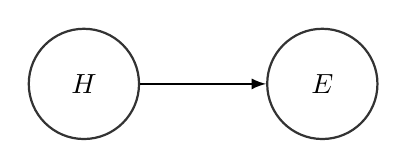
\begin{tikzpicture}
\tikzstyle{main}=[circle, minimum size = 14mm, thick, draw =black!80, node distance = 16mm]
\tikzstyle{connect}=[-latex, thick]
\tikzstyle{box}=[rectangle, draw=black!100]
  \node[main, fill = white!100] (alpha) [label=center:$H$] { };
  \node[main] (theta) [right=of alpha,label=center:$E$] { };
\path (alpha) edge [connect] (theta);
\end{tikzpicture}
\caption{Evidence and hypothesis.}
\label{fig:net}
\end{figure}

How to accommodate this evidential situation in the standard Bayesian framework? The task is: Model the learning experience. Update the agent's doxastic state accordingly. 

An natural response seems to be similar to a previous response, by expanding on the complexity of variables used. That is, we'd like a parameter to have a uniform distribution about, which then represents the agent's doxastic state towards $E$ after the learning experience. In lieu of an appropriate real-world parameter like the coin bias above, the approach here sees something like the rational or 'right' degree of belief as what the agent has a \emph{Second-Order Probability} about. A vivid advocate of this approach is Gernot D. Kleiter (e.g. in \citet{KLEITER1996143} and \citet{Pfeifer2007-PFEHRW}). The learning experience is represented by a shift of the agent's doxastic attitude in the second order from whatever prior in $E$ to a uniform distribution between 0.15 and 0.4, mirroring as closely as possible the evidential situation. It has already been argued by \citet[p.58]{Savage1954-SAVTFO-2} that such a second-order distribution merely 'collapses' into its expected value on the first-order level, and hence just complication things without contributing much, although this, of course, hasn't gone uncontested (e.g. \citet{Hansson2008-HANDWN}\footnote{Apart from their technical challenge, second order probabilities and their relation to imprecise probabilities seem to offer a lot of philosophically interesting material. This is not the place to explore them, but I'd be very interested to follow some ideas in coming papers.}) This collapsing bears a burden for second-order probabilities for the present purposes: By assuming a uniform distribution like described, one is also commited to \emph{expect} the rational probability to have a precise value. This renders pieces of information of the sort learned always comparable: If their expected values are precise, we get universal comparability again. It is unclear though, whether 'between 0.15 and 0.4' or 'between 0.2 and 0.38' describes a more probable evidential situation. This hints at the imperfect fit of the second-order model. It may be too much to postulate a uniform distribution over the interval given, since it entails equal probability of each subinterval of the same length. But, as it stands to reason, this is precisely \emph{missing} from the information learned. All we know are boundaries, we do not know about the 'inner structure' or weights of probabilities in the interval. It seems that this second-order approach goes to far and adds assumptions that go beyond the necessary, thereby losing its adequacy. 

Other approaches are either simpler (e.g. directly adopting the expected value as a precise probability and hence falling prey to the above) or leave the beaten path of orthodox Bayesianism (e.g. considering multiple Bayes net with different probability distribution / graph pairs as a doxastic attitude). It is rather compelling to conclude, therefore, that the run-of-the-mill Bayesian framework cannot account for learning this imprecise information. 

Representing the doxastic state with a set of probability functions instead of a single probability function can properly represent the evidential situation, however. To see how, we need some preliminary work. Since there are many flavours and complicated hierarchies of generality of theories discussed in the literature, as \citet{Norton2011-NORCTB} remarks, I will try and keep it simple, mainly following \citet{sep-imprecise-probabilities} and \citet{Grove:1998:USP:2074094.2074115}. We assume an algebra of propositional beliefs $\mathcal{F}$, with $\Pi$ the set of all probability functions over the according measurable space. An agents doxastic state at a given point in time is then formally represented as $\pi \subset \Pi$, that is, a set of probability functions. The learning experience can be abstractly represented as a function $U: 2^{\Pi} \times C \rightarrow 2^{\Pi}$, that is, from a set of probability functions and some conditions $C$ to a set of probability functions. How can these conditions be spelled out? First adopt the use of `summary functions', such that the degree of belief in some proposition $X$ can be described as ${\pi(X) := \{ \Pr(X) \vert \Pr \in \pi\}}$. The conditions on the learning experience then, under this interpretation, demand that $\pi'(E) = \{0.15, 0.4\}$, where $\pi'$ represents the doxastic state after the update. We could add the requirement that $\pi'(E)$ should be a convex set, and require that $\pi'(E)= [0.15,0.4]$, subject to further argument.

What does this mean for the posterior belief in $H$? In principle, this approach is not more complicated than minimizing the divergence between the posterior and prior distribution while fully respecting the constraints of the update. The difference is now that there are multiple constraints to consider. Since a single probability function cannot consistently respect both $\Pr(E) = 0.15$ and $\Pr(E) = 0.4$, we employ a single probability function for each constraint. Then we can update to $\pi'(H)$ by minimizing divergences with setting $\Pr'(E)$ to $0.15$ and to $0.4$. In this case, it amounts to Jeffrey conditionalization (citation?)

\begin{equation*} 
    \pi'(H) = \{~ \Pr(H\vert E)\text{Pr}'(E) + \Pr(H\vert\bar{E})\text{Pr}^{\prime}(\bar{E}) ~\vert~ \Pr \in \pi,~ \text{Pr}' \in \pi'~\}
\end{equation*}

Note that this is compatible with an already imprecise prior belief in $H$ as well as a precise probability, in which case $\pi(H) = \{\Pr(H)\}$.

\section{IV}

Modeling doxastic states with imprecise probabilities is not uncontroversial. Perusing the literature, I could make out two central classes of argument in favour of the use of imprecise probabilities. That is the class I dubbed `weight of evidence' on the one hand and `ignorance' on the other. While the former challenge can be met quite convincingly with the orthodox Bayesian tool box, the latter poses a more resilient problem, while they are easily dealt with using imprecise probabilities. To tip the scales further in favor of a justified use of IP, I asked: What if the evidence already is imprecise? A single sharp (second-order) probability distribution cannot account for this situation, while IP of course can. This makes a good case justifying the use of imprecise probabilities. What could staunch opponents of a narrow Bayesian framework without imprecision respond? 

First, the example given here is not much more than a parlor trick. It's requirement are exactly such as to exclude classic probabilities and cater to IP. It seems rather ad hoc. There needs to be independent and convincing motivation for the argument to go through. A concrete example from the philosophy of science would be very helpful to get the point across of \emph{why} exactly it is interesting and relevant to account for imprecise evidence. As it stands now, my research hasn't yielded very much. One way to go would be to follow the statisticians doing Robust Bayesian Analysis \citep{Berger1994} and learn more about their motivations. Maybe it is just as simple as to state that expert testimony often is vague \citep{Destercke2014}. Another route is to analyze proposals of the use of IP in quantum mechanics \citep{pittphilsci4734}, which may be promising. Unfortunately it didn't make its way into this paper yet.

Second, even if the example would be well-motivated, there is an obvious gap in the argument from `the standard Bayesian framework cannot account for this' to `we should employ IP'. The argument presupposes the absence of alternatives, but potential alternatives are heavily under explored in this paper. For example, to deal with modeling ignorance, the structurally less complex Dempster-Shafer belief functions would already be sufficient \citep{Shafer1976-SHAAMT, Norton2011-NORCTB}. The argument is in need of sharper boundaries of exactly when IP becomes a necessary addition to the philosopher's toolbox.

Third, if there really are no alternatives to IP in the given situation, it is still worth considering the problems IP bring along, in detail discussed by \citep{sep-imprecise-probabilities}, such as the oft-discussed problem of dilation, or the spurious second-order precision: the sets of probability functions have sharp boundaries. Shouldn't those be imprecise, too?  

\section{V}

Leaning imprecise information poses a problem for the orthodox Bayesian account. Switching over to an imprecise model can mitigate the problem. Of course, this is not always necessary, and prudential considerations recommend to use the simplest tool for the job. The orthodox view remains alive and well, and some careful analysis has to go into choosing and applying the right philosophical method. 


\begin{singlespacing}
\printbibliography{}
\end{singlespacing}

\end{document}
